\documentclass[11pt,a4paper]{article}
\usepackage[utf8]{inputenc}

\usepackage{geometry}
 \geometry{
 left=25mm,
 top=25mm,
 right=25mm,
 bottom=25mm,
 }
\usepackage{graphicx}	
\usepackage{bm}
\usepackage{url}
\usepackage{amsmath}	
\usepackage{todonotes}
\usepackage{verbatimbox}
\renewcommand{\baselinestretch}{1.25}

\usepackage{tikz}
\usetikzlibrary{arrows,positioning,calc}

\title{Dynamic Packet Length Control in Wireless Sensor Networks\vspace{-0.3cm}}
\author{\footnotesize  Group 42, Wireless Sensor Networks and Electronics Miniproject, June 2017\\
\footnotesize Rasmus Vestergaard, Daniel Pytlos,
Esteban Javier Struve Taguaruco,
Brynleif Andreasen and Stefan Bejan\\
\footnotesize Aarhus University, Department of Engineering}
\date{}
\begin{document}		
\maketitle

\section{Introduction}
This paper is based upon the ideas presented by Dong et al. in their study of packet length optimization schemes \cite{DPLCpaper}. They present a dynamic packet length scheme based on a lightweight link estimation method designed to capture both physical channel conditions and interference. Further, they demonstrate the effectiveness of the scheme on a testbed of TelosB motes. The purpose of the scheme is to adjust the payload size of messages, which is a change that is readily made dynamically, since it requires little extra effort from the sensors, as opposed to dynamically adjusting other factors such as bit rate or coding schemes. The reasoning behind adjusting the payload size is the fact that as packets grow larger, it is more likely that a part of the packet becomes corrupted, thus causing the packet to be dropped at the receiver. However, since the packet header has a fixed size the overhead will be larger for small packets, reducing the effective throughput. As an example, in case of TelosB motes, the radio chip CC2420 uses the IEEE 802.15.4 protocol, where the PHY+MAC headers are at least 11 bytes, depending on the adressing information contained \cite{CC2420}.

The paper is organized as follows \todo{write this + main contributions}.
\section{Packet Size Influence}
In order to understand the effects of adjusting the packet length, an analytical result is presented. First, the transmission efficiency $\mathcal{E}$, which is the amount of useful information bits received per transmitted bit, is:
\begin{equation}
\mathcal{E} = \frac{l\cdot \text{p}(l)}{l + H + O},\label{E}
\end{equation}
where $l$ is the payload length, $p(l)$ is the packet reception rate (PRR) when packets have length $l$, $H$ is overhead from the header and $O$ is additional overhead introduced by the optimization scheme. Since the scheme is not yet considered, let $O=0$ for now. Under the assumption that the channel is a Binary Symmetric Channel (BSC), the analytical value of $\mathcal{E}$ can be found. Assuming that the receiver is able to correctly detect whenever the message is incorrectly received, and has no correction capability, a packet will be passed to the higher layers only when no changes to it were introduced by the channel. The packet reception rate is then:
\begin{equation}
p(l) = (1 - p)^{l+H},
\end{equation}
where $p$ is the probability of a bit flipping in the channel. This can be used to calculate the theoretical efficiency, based on equation (\ref{E}). The result for $p=0.01$ is shown on figure \ref{fig:BSC}, with $l\in \{11,12,...,127\}$, the frame sizes possible with 802.15.4 \cite{CC2420}. It is clearly seen that there is a best efficiency $\mathcal{E}_{opt} = 0.49$ at $l_{opt} = 39$ for this specific channel. It is seen that the PRR is decreasing sharply as packet size increases. In reality, the assumption of a BSC might actually be to strict, since the BSC has an equal chance of introducing an error on any bit, whereas a burst error channel could suffer fading in an interval, causing many errors in one packet, but still only causing one packet to be dropped. This is a more difficult channel model to analyze, but it is still reasonable to conclude that longer packets will be more likely to be dropped, as the entire packet should likely be received whenever the channel is in a good state, unless the state changes during transmission.
\todo[inline]{Can add some analytical results, depending on space. Perhaps use Markov model with total of 1\% errors and calculate expected time between bursts and length of bursts - or do simulations if more accurate?}
\begin{figure}
\centering
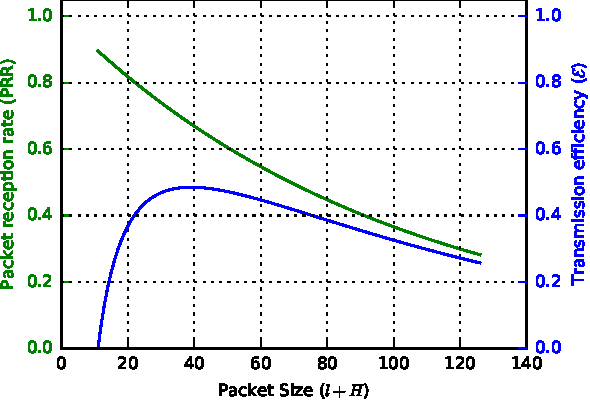
\includegraphics[scale=1]{figs/simFig_BSC001.pdf} 
\caption{\textit{Packet reception rate and Transmission efficiency for BSC with $p=0.01$.}\label{fig:BSC}}
\end{figure}
\section{Estimating the Channel\label{sec:chanEst}}

The first experiment performed had the purpose of estimating the channel properties in different conditions. For this experiment, no dynamic packet length control scheme was used. Instead, simple, out-of-the box packet transmission  with different packet lengths has been used. Based on the number of received packages, the PRR $p(l)$ and efficiency $\mathcal{E}$ have been estimated.

\paragraph{Transmitter} The transmitter sends a fixed number of packets to the receiver. The length of the packets decreases gradually in steps of $10$ bytes. In our implementation the transmitter sends $1000$ packages periodically, every 50 milliseconds, starting with the maximum $l = 100$. After the first batch of messages has been sent, the transmitter waits $5$ seconds before sending the next batch of (smaller) packets.

\paragraph{Receiver} The receiver is slightly less complicated as it's only role is to count the number of received messages and to periodically report this counter together with the current received payload length $l$ to a computer, using the serial connection. In our implementation, this happens every $2$ seconds.

\paragraph{}With the information provided by the receiver, the Packet Reception Rate $PRR$ and transmission efficiency $\mathcal{E}$ are calculated using a \textsc{python} script. The results for the channel where the distance between the motes was $35$ meters can be seen in figure \ref{fig:35mTest} and for the $45$ meters distance in figure \ref{fig:45mTest}. For the channel between the motes placed at $35$ meters, it can be seen that the maximum transmission efficiency $\mathcal{E}$ is reached when they payload is about $80$ bytes. Even though the measurements for the channel where the distance between the motes was $45$ meters present a lot of variation, it is possible to see that the efficiency reaches a maximum at a lower packet size $l$ ($50-80$ bytes). This result is expected as the distance between the motes deteriorates the quality of the channel and increases the probability of bit error - therefore the probability of corrupting a larger packet.

\paragraph{} The results presented show the relationship between distance and transmission efficiency of the channel. We use these results in order to verify that the DPLC scheme implemented functions as expected, choosing the a dynamic packet length that maximizes the capacity of the channel. The comparable results we obtained when using the DPLC scheme are presented in section \ref{sec:schemeTest}.

\begin{figure}
\centering
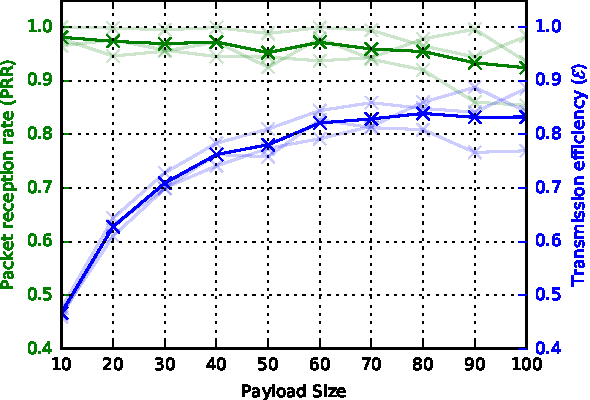
\includegraphics[scale=1]{figs/35mTest.pdf} 
\caption{\textit{PRR and transmission efficiency, 35 meters apart}\label{fig:35mTest}}
\end{figure}

\begin{figure}
\centering
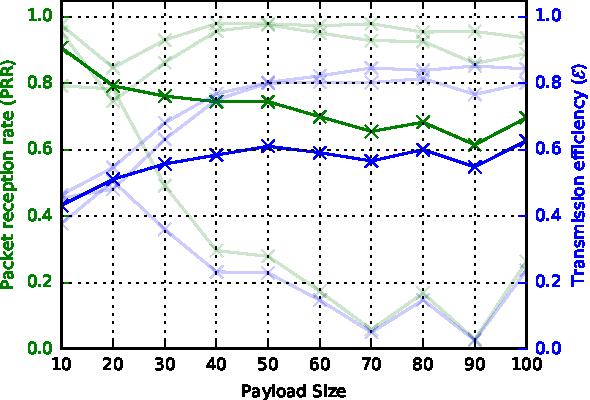
\includegraphics[scale=1]{figs/45mTest.pdf} 
\caption{\textit{PRR and transmission efficiency, 45 meters apart}\label{fig:45mTest}}
\end{figure}
\section{Dynamic Packet Length Control Scheme\label{sec:DPLC}}
It is now established that the payload length chosen has a significant influence on the resulting transmission efficiency. This section describes a simple scheme that allows a mote to dynamically adjust the payload size and continously maximize the transmission efficiency based on current channel conditions. Define the parameters at time instance $i$: 
\begin{equation}
(\mathcal{E}_i , l_i) \coloneqq (\mathcal{E}(l_i) , l_i).
\end{equation}
At a given time $k-1$, the sequence of previous parameters can be used to estimate what the payload length should be at time $k$:
\begin{equation}
l_k = f\left(
(\mathcal{E}_i , l_i )_{i=0}^{k-1}
\right),
\end{equation}
where $f(\cdot)$ is a function to calculate the new payload length based on the previous ones. In reality, all previous parameters cannot be used for multiple reasons: First, the wireless channel is known to be time-varying and a given relationship between packet length and transmission efficiency cannot be expected to be similar to what was observed earlier, if a long period of time has passed. Second, the sensor motes usually have severely constrained storage, and storing all old information could take a large part of the available memory. Therefore, a scheme using only the previously described parameters is designed. Assuming that the channel estimation is performed frequently, it is expected that there will be a high correlation between subsequent time slots. The channel estimation is achieved in as described in section \ref{sec:chanEst}. The transmitting mote records the number of packets it has sent, and periodically asks the receiving mote how many packets it has received. In this way, the packet reception rate is estimated and used by the receiving mote to calculate the channel efficiency at time $i$, $\mathcal{E}_i$. Two gradient variables are defined, calculated from the current and previous parameters obtained:
\begin{align}
\Delta \mathcal{E} &\coloneqq (\mathcal{E}_i - \mathcal{E}_{i-1}),\\
\Delta l &\coloneqq (l_i - l_{i-1}).
\end{align}
These first gradient variable, $\Delta \mathcal{E}$, captures the change in transmission efficiency introduced by adjusting the payload length from $l_{i-1}$ to $l_{i}$: If $\Delta \mathcal{E} > 0$ the change improved the efficiency, whereas a $\Delta \mathcal{E} < 0$ indicates a decline. The other variable captures what the last change in payload length was: If $\Delta l > 0$ the payload length was increased last, and $\Delta l < 0$ shows that the payload length was decreased last. Based on these two parameters a direction variable, $d$ is calculated, and used for determining what change needs to be made to the payload length:
\begin{equation}
d = \Delta \mathcal{E}\cdot\Delta l,\label{eq:d}
\end{equation}
where it is clear that there are four distinct options:
\begin{itemize}  
\setlength{\itemsep}{1pt}
\setlength{\parskip}{0pt}
\setlength{\parsep}{0pt}
\item[ ] $\Delta l < 0 \wedge \Delta \mathcal{E} < 0 \Rightarrow d > 0$\quad \textit{(Worse efficiency from smaller payload)},
\item[ ] $\Delta l < 0 \wedge \Delta \mathcal{E} > 0 \Rightarrow d < 0$\quad \textit{(Better efficiency from smaller payload)},
\item[ ] $\Delta l > 0 \wedge \Delta \mathcal{E} < 0 \Rightarrow d < 0$\quad \textit{(Worse efficiency from larger payload)},
\item[ ] $\Delta l > 0 \wedge \Delta \mathcal{E} > 0 \Rightarrow d > 0$\quad \textit{(Better efficiency from larger payload)}.
\end{itemize}
The next payload length is chosen based on the resulting value of $d$. If $d$ is positive, the payload length should be increased, whereas a negative value for $d$ means that the payload length should be decreased. In order to allow the scheme to reach a steady state, it is determined that a threshold $\pm D$ should be exceeded for a change to be made in the channel, i.e. $|d| > D$. Further, only changes of $\pm 10$ bytes are allowed to the payload length, in order to make changes that are large enough to be significant, yet small enough for the efficiency to be correlated to the previous estimate. Figure \ref{fig:d} summarizes what the effect a given value of $d$ has on the payload length.
A special case arises when the parameter $d$ falls between the thresholds, i.e. $|d| < D$. In this case, there is no change to the packet length. The effect of this is that in the next timestep $\Delta l= 0$, thus causing $d = 0$ according to equation (\ref{eq:d}). This causes a steady state, where the payload length will not change anymore. As the channel conditions could easily change after a steady state has been reached, it is determined that after a certain number of time steps with no change in the payload length, a change is forced to cause the scheme to search for a new optimum.
The change is forced as $l_i = l_{i-1} + 10$, an addition of ten bytes to the payload length, unless the payload length is already at the maximum allowed for the scheme, where the change will be $l_i = l_{i-1} -10$, a subtraction of ten bytes instead. The reason for automatically forcing an increase rather than a decrease is to be greedy: If the payload length is bigger the overhead from the header is smaller, thus it is desirable to immediately increase the payload length if the channel conditions have become better that it was when the steady state was reached. The end for a dynamic scheme is to adapt to changing conditions, searching for the parameter that can maximize the throughput of the link. If the channel conditions instead became worse, the scheme would adapt to this, and reduce the payload length at the next time step. 
\begin{figure}
\centering
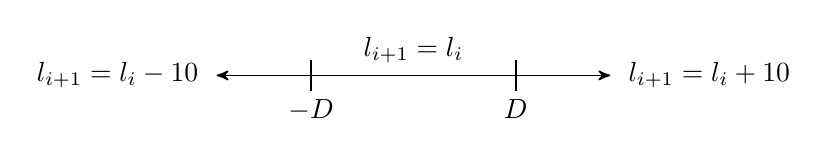
\begin{tikzpicture}[->, >=stealth', auto, semithick, node distance=3cm]
\centering
\draw[<->,line width=0.6pt] (0,0) node[left=3pt] {$l_{i+1} = l_i - 10$} -- node[above=1pt] {$l_{i+1} = l_i$} (5,0.0) node[right=3pt] {$l_{i+1} = l_i + 10$};
\draw[-,line width=0.6pt] (1.2,0.2) -- node[below=5pt]{$-D$}(1.2,-0.2);
\draw[-,line width=0.6pt] (3.8,0.2) -- node[below=5pt]{$D$}(3.8,-0.2);
\end{tikzpicture}
\caption{\textit{The value of $d$ determines the next packet length, according to predefined intervals.}\label{fig:d}}
\end{figure}
\section{Conclusion\label{sec:conclusion}}
Wireless Sensor Networks (WSNs) present a real challenge in the industry as more emphasis is put on pervasive computing paradigms. However, a constant trade-off between efficiency, power consumption, scalability and ease of deployment needs to be achieved, depending on the individual usage scenarios. One often important factor is the reliability of communication between the the sources and the sinks. Reliability can be increased by using error control schemes or retransmissions of packets. However, these approaches might be inappropriate for some setups where the sensors have power constraints or inadequate hardware capabilities. 
In order to reduce the strain on motes in the network, it would be beneficial to increase the transmission efficiency, which is the ratio of received, useful bits to the number of total transmitted bits. One way to od this is by adjusting the packet length. This is because, as the channel introduces noise, the packets with a larger size have a higher probability of getting corrupted and lost. Small packets have a larger overhead in terms of the header, so there is thus a trade-off.
\\[8pt]
This paper has investigated the possibility of dynamically adjusting the packet length based on the quality of the channel in order to maximize its throughput. Initially, it was established that the size of packets transmitted indeed do influence the transmission efficiency. It was shown analytically for a Binary Symmetric Channel, as well as experimentially in an indoor environment. Then, a scheme was applied that would give sensor motes the capability to dynamically adjust their transmission packet length based on the estimated current link quality, in order to continously maximize transmission efficiency, was presented. This scheme was verified through both simulations and test in a real scenario, where the scheme was implemented on TelosB motes. The results show that the scheme are able to adapt to channel conditions in the setup demonstrated. 
%\\[1cm]
%In section \ref{sec:intro}, the challenge and the purpose of the report has been stated. Section \ref{sec:pacSizeInf} presented the basic theoretical background for adjusting the packet length and how this influences the capacity of the Binary Symmetric Channel (BSC). In section \ref{sec:chanEst} the application of theory from section \ref{sec:pacSizeInf} was considered and the results obtained without usage of dynamic packet length control (DPLC) were shown. Section \ref{sec:DPLC} introduced a theoretical proposal for dynamically adjusting packet length and in section \ref{sec:simScheme}, theoretical scheme simulation results were presented and analyzed. In section \ref{sec:schemeTest}, the real implementation of the DPLC scheme was demonstrated and the results interpreted. Further work that could improve the overall quality and capacity of the implementation were presented in section \ref{sec:FW}.
\\[8pt]
In conclusion, the principles presented in the article by Dong et al. \cite{DPLCpaper} are useful, and adjusting the transmission packet length is a feasible way to optimize transmission efficiency in wireless sensor networks. This is thus yet another factor that may be considered when optimizing a wireless sensor network for a particular application. The work presented in this paper has been purely scientific, and in order to utilize the scheme in an actual scenario, several issues must be dealt with, and choices made. Some of these issues were reflected upon in the paper.
%\\[8pt]
%Considering the results presented in this paper, we can conclude that even though our implementation could have been a lot more advanced, it was enough to prove the points presented in the article by Dong et al. \cite{DPLCpaper} and to motivate further research on the topic of dynamic length packet control. 

\nocite{*}
\bibliography{refs}
\bibliographystyle{ieeetr}
\end{document}